\section{Elliptic Curves}

% ------------------------------- %
% DEFINITION AND BASIC PROPERTIES %
% ------------------------------- %
\subsection{Definition and basic properties}
\label{subs:definition-properties}

We now have all the prerequisites to define what an elliptic curve is.
\begin{definition}
	An \emph{elliptic curve} is a smooth curve $E$ of genus 1 with a specified point
	$O \in E$.
\end{definition}
We will see later that $E$ can be given the structure of a group, which is the
reason why we
specify a point $O$, which will act as the identity element.

\begin{remark}
	From \ref{cor:genus-formula}, we get that any smooth cubic
	plane curve with a specified point $O$ is an elliptic curve.
\end{remark}

A \emph{Weierstrass equation} is an equation of a 
cubic plane curve $C \subset \proj^2$ of the form
\begin{equation*}
	Y^2Z + aXYZ + bYZ^2 = X^3 + cX^2Z + dXZ^2 + eZ^3.
\end{equation*}
We can consider the set $U_Z = \{Z \neq 0\} \subset \proj^2$. We have that
$C \cap U_Z$ is an affine curve for which the set of points
$[X, Y, 1] \in C\cap U_Z$ is specified by the dehomogenized equation
\begin{equation*}
	Y^2 + aXY + bY = X^3 + cX^2 + dX + e.
\end{equation*}
To ease notation, we will 
use the dehomogenized equation to define the projective curve $C$,
remembering that there is the point at infinity $[0, 1, 0]$.

We will see that any elliptic curve can be, up to isomorphism, 
characterized by a Weierstrass equation. Before proving this, we will need
the following lemma about singular curves given by a 
Weierstrass equation.
\begin{lemma}
	\label{lem:deg-1-singular}
	If a curve $C$ given by a Weierstrass equation is singular,
	then there exists a rational map $\phi:E \to \proj^1$ of degree 1.
\end{lemma}

\begin{proof}
	Making a linear change of variables, we may assume that the singular point
	is $(x, y) = (0, 0)$. By checking the partial derivatives, we have that
	the Weierstrass equation is of the form
	\begin{equation*}
		C: y^2 + axy = x^3 + cx^2.
	\end{equation*}
	The rational map
	\begin{equation*}
		\phi: E \to \proj^1, (x, y) \mapsto [x, y]
	\end{equation*}
	Induces an isomorphism
	\begin{equation*}
		\phi: U \to V
	\end{equation*}
	Where $U = E\setminus\{[0, 0, 1], [0, 1, 0]\} \subset E$
	and $V = \proj_1\setminus\{[1, 0], [0, 1]\} \subset \proj^1$
	with inverse given by $[1, t]\mapsto(t^2 + at - c, t^3 + at^2 - ct)$
	(indeed, if we set $t = \frac{y}{x}$, and note that if we divide the
	equation for $C$ by $x^2$, we obtain $t^2 + a_1t = x+ a_2$, so
	$\phi(x, y) = [1, t]$ is indeed mapped to $[x, tx] = [x, y]$)
	Hence $\phi$ induces an isomorphism of function fields
	$\phi^*: K(V) \to K(U)$ and hence
	$\phi^*: K(\proj^1) \to K(E)$ is an isomorphism 
	(since $K(V) = K(\proj^1)$ and $K(U) = K(E)$).
	It follows that $\deg\phi = 1$.
\end{proof}

% ELLIPTIC CURVE ADMITS A WEIERSTRASS EQUATION

The following proposition allows us to identify elliptic curves
with smooth curves given by a Weierstrass equation.
\begin{proposition}
	\label{prop:curve-correspondence}
	Let $(E, O)$ be an elliptic curve defined over $K$.
	\begin{enumerate}[itemsep=0em, label=(\alph*)]
		\item There exist functions $x, y \in K(E)$ such that the map
			\begin{align*}
				\phi: E &\to \proj^2\\
				P &\mapsto [x(P), y(P), 1]
			\end{align*}
			gives an isomorphism of $E$  onto a curve given by 
			the Weierstrass equation
			\begin{equation*}
				C: Y^2 + aXY + bY = X^3 + cX^2 + dX + e
			\end{equation*}
			with coefficients $a, b, c, d, e \in K$ and such that $\phi(O) =
			[0,1, 0]$. We call $x, y$ the Weierstrass coordinate functions
			on $E$.
		\item Any two equations for $E$ as in (a) are related by a linear change
			of variables of the form
			\begin{align*}
				X &= u^2X' + r\\
				Y &= u^3Y' + su^2X' + t
			\end{align*}
			with $u, r, s, t \in K, u \neq 0$.
	\end{enumerate}
\end{proposition}

\begin{proof}
	Consider the vector spaces $\L(n\,(O))$ for $n \in \N$.
	By the Riemann-Roch theorem, since elliptic curves have genus 1,
	\begin{equation*}
		l(n\,(O)) = \dim(\L(n\,(O))) = \deg(n\,(O)) = n
	\end{equation*}
	for all $n \geq 1$. Hence we can choose $x, y \in K(E)$, such that
	$\{1, x\}$ is a basis for $\L(2\,(O))$ and $\{1, x, y\}$
	is a basis for $\L(3\,(O))$.
	Since $x \in \L(2\,(O))\setminus\L((O))$, 
	and $y \in \L(3\,(O))\setminus\L(2\,(O))$, we have that
	$x$ and $y$ have poles at $O$ of exact order $2$ and $3$
	respectively.
	
	Now, $\L(6\,(O))$ is of dimension $6$, but it contains the seven
	functions $1, x, y, x^2, xy, y^2, x^3$ (which we see easily by
	looking at the order of the pole at $O$). Hence there has to be some
	linear relation
	\begin{equation*}
		A_1 + A_2x + A_3y + A_4x^2 + A_5xy + A_6y^2 + A_7x^3 = 0,
	\end{equation*}
	with the $A_i$ not all zero.
	Since $1, x, y, x^2, xy$ all have a pole of different order at $O$,
	we have necessarily that $A_6$ and $A_7$ are non-zero.
	We replace $x$ by $-A_6A_7x$ and $y$ by $A_6A_7^2y$, then if we divide 
	the equation by $A_6^3A_7^4$, we obtain an equation in the Weierstrass
	form. This equation describes a curve in which lies the image of the map
	\begin{align*}
		\phi:E &\to \proj^2\\
		P &\mapsto [x(P), y(P), 1]
	\end{align*}
	By definition, $\phi$ is a morphism, furthermore, it is not constant,
	so it is surjective. Furthermore, $\phi(O) = [0, 1, 0]$, since
	$y$ has a higher order pole than $x$ at $O$.

	We will now show that the map $\phi: E\to C\subset \proj^2$ is of degree 1.
	We have that
	\begin{equation*}
		\deg\phi = [K(E): \phi^*K(C)] = [K(E): K(x, y)]
	\end{equation*}
	Consider the map $[x, 1]: E \to \proj^1$. Since $x$ has a double pole
	at $(O)$ and no other poles, we have that (using that
	$Y/X$ is a uniformizer of $\O_{[1, 0]}(\proj^1)$)
	\begin{align*}
		\deg[x, 1] &= \sum_{P \in [x, 1]^{-1}([1, 0])}
		e_{[x, 1]}(P)\\
		&= e_{[x, 1]}(O)
		= \ord_O(1/x) = 2.
	\end{align*}
	Hence we get $[K(E): K(x)] = 2$.
	
	Similarly,
	we deduce that $[y, 1]: E \to \proj^1$ 
	has degree 3, and hence $[K(E): K(y)] = 3$.
	It follows that $[K(E): K(x, y)] = 1$ since $\gcd(2, 3) = 1$.
	Hence $K(E) = K(x, y)$ and so $\phi$ has degree 1.

	Suppose ad absurdum that $C$ is singular, then \ref{lem:deg-1-singular}
	yields a rational map $\psi: C \to \proj^1$ of degree 1. Hence
	the composition $\psi\circ\phi: E \to \proj^1$ is a map of degree 1 between
	smooth curves and hence an isomorphism (\ref{cor:deg-1-isom}).
	This contradicts the fact that $E$ has genus 1 and $\proj^1$ has genus 0
	(\ref{ex:proj-genus}). Hence $C$ is smooth, so again by
	\ref{cor:deg-1-isom},
	we have that the degree 1 map $\phi: E \to \C$ is
	an isomorphism, which proves part (a).

	For part (b), suppose we have two pairs of Weierstrass coordinate functions
	$(x, y)$ and $(x', y')$, then $x$ and $x'$ have poles of order 2 at $O$
	and $y$ and $y'$ have poles of order 3 at $O$.
	Hence $\{1, x\}$ and $\{1, x'\}$ are two bases for $\L(2\,(O))$
	and $\{1, x, y\}$ and $\{1, x', y'\}$ are two bases for
	$\L(3\,(O))$. We deduce that there are some constants
	$u_1, u_2, r, s_2, t \in K$ with $u_1u_2 \neq 0$ such that
	\begin{equation*}
		x = u_1x' + r\qquad\textrm{and}\qquad y= u_2y' + s_2x' + t
	\end{equation*}
	But since both $(x, y)$ and $(x', y')$ satisfy Weierstrass equations in
	which the $Y^2$ and $X^3$ terms have coefficient $1$, we deduce that
	$u_1^3 = u_2^2$. So letting $u = u_3/u_1$ and $s = s_2/u^2$, puts the change
	of variables into the desired form.
\end{proof}

% WEIERSTRASS EQUATION CAN BE SIMPLIFIED

Now, let $E$ be an elliptic curve defined by the Weierstrass equation
\begin{equation}
	\label{weierstrass-eq}
	E: Y^2 + aXY + bY = X^3 + cX^2 + dX + e
\end{equation}
for some $a, b, c, d, e \in K$ with origin $O = [0, 1, 0]$.

When $\chr(K) \not\in \{2, 3\}$ (recall we assumed this is true throughout this
paper), we can simplify (\ref{weierstrass-eq}) using changes of variables,
if we set $Y = Y' - \frac{1}{2}(aX'  + b)$ we obtain an equation of the form
\begin{equation*}
	Y'^2 = X^3 + c'X^2 + d'X + e'
\end{equation*}
with $c', d', e' \in K$. We can also get rid of the term $X^2$ with the
substitution $X = X' - \frac{1}{3}c'$, we obtain an equation of the form
\begin{equation*}
	Y'^2 = X'^3 + AX' + B
\end{equation*}
with $A, B \in K$. A quick calculation yields $c' = c + \frac{1}{4}a^2$,
hence up to using the linear change of variables
\begin{align*}
	X &= X' - \frac{1}{3}\left(c  + \frac{1}{4}a^2\right),\\
	Y &= Y' - \frac{1}{2}(aX'  + b),
\end{align*}
we can always suppose an elliptic curve $E$ is given by the equation
\begin{equation*}
	E: Y^2 = X^3 + AX + B.
\end{equation*}

% CONDITION FOR CURVE BEING SINGULAR

From \ref{prop:curve-correspondence}, we know that a curve given by the an equation
of the above form is an elliptic curve whenever it is smooth.
The following proposition answers the question of when that is the case.
\begin{proposition}
	\label{prop:singular-determinant}
	Let $C$ be a projective plane curve defined by
	\begin{equation*}
		C: F(X, Y) = X^3 + AX + B - Y^2 = 0.
	\end{equation*}
	Let $\Delta = 4A^3 + 27B^2$ be the discriminant of $F(X, 0)$, then 
	$C$ is smooth (and hence an elliptic curve)
	if and only if $\Delta \neq 0$.
\end{proposition}
\begin{proof}
	First, let us verify that $O = [0, 1, 0]$ is not singular.
	If we look at $C$ in the chart $U_Y = \{Y \neq 0\}$, we get
	that $C$ is given by the equation
	\begin{equation*}
		G(X, Z) = X^3 + AXZ^2 + BZ^3 - Z = 0.
	\end{equation*}
	We have that
	\begin{equation*}
		\nabla G(0, 0) =
		\begin{bmatrix}
			0\\
			1
		\end{bmatrix} \neq 0,
	\end{equation*}
	and so $O$ is a smooth point of $C$.
	
	Suppose there is a point $P = (x, y) \in C$ that is singular,
	then we have
	\begin{equation*}
		\nabla F(P) =
		\begin{bmatrix}
			3x^2 + A\\
			-2y\\
		\end{bmatrix} = 0
	\end{equation*}
	Hence we have that $\frac{\partial}{\partial X}F(x, 0) 
	= 3x^2 + A = 0$.
	In particular, since $P \in C$, also 
	$F(x, 0) = 0$, and hence
	$x$ is a double root of $F(X, 0)$ so we deduce that the discriminant
	$\Delta = 4A^3 + 27B^2$ is zero.

	Suppose instead that $\Delta = 0$, then $F(X, 0)$ admits a double root
	$x \in K$ (recall $K$ is algebraically closed).
	Then $P = (x, 0) \in C$ and
	\begin{equation*}
		\nabla F(P) =
		\begin{bmatrix}
			3x^2 + A\\
			0\\
		\end{bmatrix} = 0,
	\end{equation*}
	since $3x^2 + A = \frac{\partial}{\partial X}F(x, 0) = 0$.
	It follows that $C$ is singular at $P$.
\end{proof}

% ---------
% GROUP LAW
% ---------
\subsection{Group Law}

In this section, we will endow elliptic curves with a group structure.
Usually, the composition law is defined geometrically for cubic plane curves.
To stay as general as possible, we will first define the composition law
using the degree 0 part of the divisor class group and then show that
the two group laws are the same.

\begin{proposition}
	Let $(E, O)$ be an elliptic curve. The map
	\begin{align*}
		\kappa: E &\to \Cl^0(E)\\
		P &\mapsto \cl{(P) - (O)}
	\end{align*}
	is a bijection.
\end{proposition}

\begin{proof}
	Let $D \in \Div^0(E)$ be a divisor. Since $E$ has genus 1, 
	by the Riemann-Roch theorem (\ref{thm:riemann-roch}), we have that
	\begin{equation*}
		\dim\L(D + (O)) = 1.
	\end{equation*}
	Let $f \in K(E)$ be a generator for $\L(D + (O))$. Since
	\begin{equation*}
		\div(f) \geq -D -(O)
		\quad\textrm{ and }\quad
		\deg(\div(f)) = 0,
	\end{equation*}
	we have necessarily that 
	\begin{equation*}
		\div(f) = -D -(O) + (P)
	\end{equation*}
	for some $P \in E$.
	Hence 
	\begin{equation*}
		D \sim (P) - (O).
	\end{equation*}
	Suppose there is some other $P' \in E$, such that $D \sim (P') - (O)$.
	Then $(P) \sim (P')$, but then $P = P'$ from \ref{prop:sim-implies-eq}.
	
	This allows us to define
	\begin{equation*}
		\sigma: \Div^0(E) \to E,
	\end{equation*}
	which sends a divisor $D \in \Div^0(E)$ to the corresponding point $P \in E$
	as above.

	This map is clearly surjective, as $\sigma((P) - (O)) = P$. Furthermore, we
	have that $\sigma(D_1) = \sigma(D_2)$ if and only if $D_1 \sim D_2$.
	Indeed, if $D_1 \sim D_2$, then 
	\begin{equation*}
		(\sigma(D_1)) - (O) \sim D_1 \sim D_2 \sim (\sigma(D_2)) - (O)
	\end{equation*}	
	and hence $\sigma(D_1) = \sigma(D_2)$ by \ref{prop:sim-implies-eq}.
	Conversely, if $\sigma(D_1) = \sigma(D_2)$, then clearly
	\begin{equation*}
		D_1 \sim (\sigma(D_1)) - (O) = (\sigma(D_2)) - (O) \sim D_2.
	\end{equation*}
	We deduce that $\sigma$ induces a bijection $\widehat{\sigma}: \Cl^0(E) \to E$.
	Furthermore, clearly $\widehat{\sigma} = \kappa^{-1}$.
\end{proof}

% DEFINITION OF GROUP LAW

Using $\kappa$, we can define the composition law $+$ as the unique
composition law, which makes $\kappa$ a group isomorphism.
In particular, this gives $E$ the structure of an abelian group
with identity element $O = \kappa^{-1}(0)$,
\begin{definition}
	We define the composition law $+$ on $(E, O)$, by 
	\begin{equation*}
		P + Q = \kappa^{-1}(\kappa(P) + \kappa(Q))
	\end{equation*}
	for all $P, Q \in E$.
\end{definition}

\begin{notation}
	For $m \in \N\setminus\{0\}$ and $P \in E$ we define
	\begin{equation*}
		[m]P = \underbrace{P + \dots + P}_{m\textrm{ times}}.
	\end{equation*}
	We extend this definition to $m \in \Z$ with $[0]P = O$ and
	$[m]P = [-m](-P)$ for $m < 0$.
\end{notation}

% CRITERIA PRINCIPAL DIVISORS

Thanks to how the composition law is defined on $E$, we get the following
criteria that tells us when a divisor is principal.
\begin{proposition}
	\label{prop:div-principal}
	Let $(E, O)$ be an elliptic curve and $D = \sum n_P \cdot (P) \in \Div(E)$.
	Then $D$ is principal if and only if $\sum n_P = 0$ and $\sum [n_P]P = O$
\end{proposition}

\begin{proof}
	Suppose $D$ is principal, so $D\sim 0$. 
	Principal divisors have degree $0$,
	hence $\sum n_P = 0$. It follows that
	\begin{align*}
		\kappa\left(\sum [n_P]P\right) &= \sum n_P\kappa(P) = \sum n_P
		\cdot\cl{(P) - (O)}\\
		&= \cl{\sum n_P\cdot(P)} = 0
	\end{align*}
	And hence $\sum [n_P]P = 0$ by injectivity of $\kappa$.

	Now suppose $\sum n_P = 0$ and $\sum [n_P] P = O$,
	then by the above calculation,
	\begin{equation*}
		\cl{D} = \cl{\sum n_P\cdot(P)} = \kappa\left(\sum [n_P] P\right) = 0
	\end{equation*}
	and so $D \sim 0$.
\end{proof}

% GEOMETRIC COMPOSITION LAW

We will now introduce another composition law defined for smooth cubic plane
curves and show that it coincides with the group law induced from $\Cl^0(E)$.
This will not only provide the link with the usual definition of composition
on an elliptic curve, but also give another way to compute the sum
of two points on an elliptic curve.

Let $E$ be a smooth cubic plane curve.
By Bézout's theorem, for any line $L \subset \proj^2$, $L$ intersects
$E$ in exactly 3 points (taken with multiplicity).
This allows us to define a composition law $\oplus$ on $E$ as
follows.

\begin{definition}
	\label{def:group-law}
	Let $P, Q \in E$ and $L$ the line connecting $P$ and $Q$ (or the tangent line
	to $E$ at $P$ if $P = Q$). Let $R$ be the third point of intersection of $L$
	with $E$. Let $L'$ be the line connecting $R$ and $O$. We define $P \oplus Q$
	be the third point of intersection of $L'$ with $E$.
\end{definition}

\begin{figure}[ht]
	\centering
	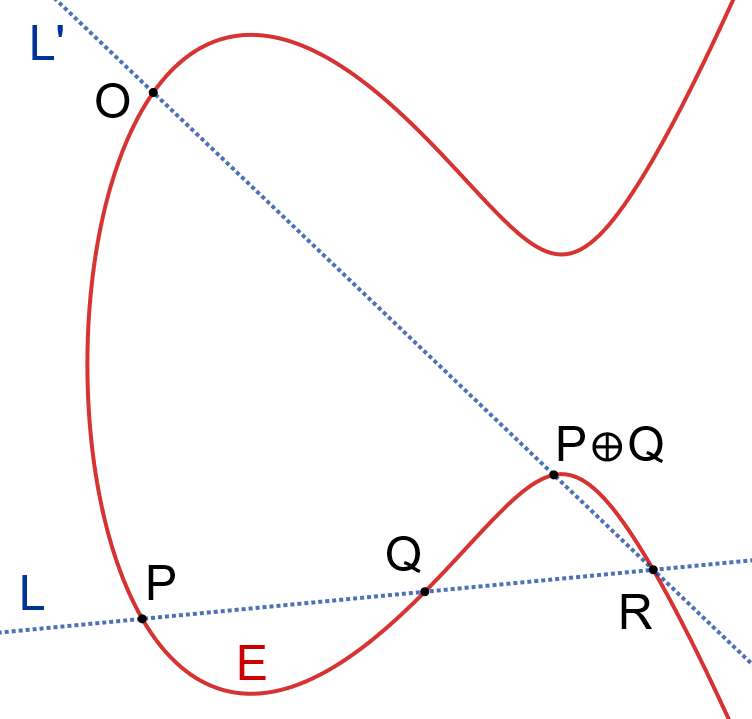
\includegraphics[width=0.5\textwidth]{addition}
	\caption{Visualization of geometric composition law}
\end{figure}

% EQUIVALENCE OF COMPOSITION LAWS

\begin{proposition}
	\label{prop:equivalence-composition}
	Let $E$ be a smooth cubic plane curve, then for all $P, Q \in E$,
	\begin{equation*}
		P \oplus Q = P + Q.
	\end{equation*}
\end{proposition}

\begin{proof}
	We have to show that for $P, Q \in E$,
	$\kappa(P \oplus Q) = \kappa(P) + \kappa(Q)$.

	Let
	\begin{equation*}
		f(X, Y, Z) = \alpha X + \beta Y + \gamma Z = 0
	\end{equation*}
	give the line $L$ in $\proj^2$ going through $P, Q$ and let $R$ be the third
	point of intersection.
	Let $g(X, Y, Z) = 0$ be the equation for the tangent line $T$ to
	$E$ at $O$. $T$ intersects $E$ at $O$ with
	multiplicity at least 2, let $S \in E$ be the third point of intersection
	(equal to $O$ if $O$ is a flex).
	Since $g$ is homogeneous of degree 1, $f/g \in K(E)$ and so we get that
	\begin{align*}
		\div(f/g) &= \sum_{P' \in E}\ord_{P'}(f)\cdot(P')
		- \ord_{P'}(g)\cdot(P')\\
		&= \sum_{P' \in E}I(P', E\cap L)\cdot(P') - I(P', E\cap T)\cdot(P')\\
		&= (P) + (Q) + (R) - 2(O) - (S).
	\end{align*}
	Now let 
	\begin{equation*}
		f'(X, Y, Z) = \alpha' X + \beta' Y + \gamma' Z = 0
	\end{equation*}
	be the line $L'$ through $R$ and $O$. Then by the definition of $\oplus$,
	we have that the third point of intersection of $L'$ with $E$ is 
	$P \oplus Q$. As above, $f'/g \in K(E)$ and we have
	\begin{equation*}
		\div(f'/g) = (R) + (O) + (P \oplus Q) - 2(O) - (S)
		= (R) + (P + Q) - (O) - (S).
	\end{equation*}
	It follows that
	\begin{equation*}
		\div(f'/f) = \div(f'/g) - \div(f/g) = (P \oplus Q) - (P) - (Q) + (O)
	\end{equation*}
	And hence
	\begin{align*}
		\kappa(P \oplus Q) - \kappa(P) - \kappa(Q) &= 
		\cl{(P \oplus Q) - (O)} - \cl{(P) - (O)} - \cl{(Q) - (O)}\\
		&= \cl{(P \oplus Q) - (P) - (Q) + (O)} = 0.
	\end{align*}
\end{proof}

\begin{remark}
	As a byproduct of the equivalence of $+$ and $\oplus$, we get
	essentially for free that $E$ with the geometric composition law $\oplus$
	satisfies the group axioms (for example, from the definition of
	$\oplus$ it is not clear at all why this composition law should be
	associative).
\end{remark}

% EXPLICIT FORMULAS FOR ADDITION

Thanks to the equivalence of $+$ and $\oplus$, we can calculate explicit
formulas for addition on $E$. As we have seen in
Section \ref{subs:definition-properties}, we can suppose up to a curve isomorphism
that $E$ is given by the reduced Weierstrass equation
\begin{equation*}
	E: F(x, y) = y^2 - x^3 - ax - b = 0
\end{equation*}
with origin $O = [0, 1, 0]$.

Let $P = (x_P, y_P) \in E$, then we
\begin{equation*}
	-P = (x_P, -y_P).
\end{equation*}
Indeed, the line connecting $P$ and $(x_P, -y_P)$, is the line
$X = x_PZ$, which has as third intersection point $O$.
The tangent to $E$ at $O$ is given by $Z = 0$,
which intersects $E$ with multiplicity 3 at $O$,
hence we obtain that $P+(x_P, -y_P) = O$.

Now let $Q = (x_Q, y_Q) \in E$ different from $-P$. Then $P + Q \neq O$.
Suppose $P \neq Q$, then $x_P \neq x_Q$. 
We have that the line passing through $P$ and $Q$ is given by
\begin{equation*}
	L: y = \frac{y_Q - y_P}{x_Q - x_P}(x - x_P) + y_P
\end{equation*}
Setting 
\begin{equation*}
	\lambda = \frac{y_Q - y_P}{x_Q - x_P}
	\quad\textrm{ and }\quad
	\nu = \frac{x_Qy_P - x_Py_Q}{x_Q - x_P}
\end{equation*}
we can rewrite $L: y = \lambda x - \nu$.

If $P = Q$, then $L$ is the tangent to $E$ at $P$, which is given by
\begin{equation*}
	L: (3x_P^2 + a)(x - x_P) - 2y_P(y - y_P) = 0
\end{equation*}
Suppose ad absurdum that $y_P = 0$,
then $L$ is the line $x = x_P$ (the term $3x_P^2 + a$ is non-zero, since
$E$ is not singular) and so the third point of intersection
is $O$, whence $P + Q = O$, which contradicts our assumption, and so 
$y_P \neq 0$.
To obtain again an equation of the form $L = \lambda x - \nu$, we have to set
\begin{equation*}
	\lambda = \frac{3x_P^2 + a}{2y_P}
	\quad\textrm{ and }\quad
	\nu = \frac{-3x_P^3 - ax_P + 2y_P^2}{2y_P}
	= \frac{-x_P^3 + ax_P + 2b}{2y_P}.
\end{equation*}

So let $\lambda$ and $\nu$ be as above corresponding to the case.
Let $R$ be the third point of intersection of $L$ with $E$.
We have that the equation $F(x, \lambda x + \nu) = 0$ with respect to $x$
admits exactly the zeroes $x_P, x_Q, x_R$ and hence
\begin{equation*}
	F(x, \lambda x + \nu) = c(x - x_P)(x - x_Q)(x - x_R)
\end{equation*}
Since the coefficient of $x^3$ in $F(x, \lambda x + \nu)$ is $-1$, we obtain
$c = -1$. By equating the coefficient of $x^2$, we obtain
$\lambda^2 = x_P + x_Q + x_R$ and hence
\begin{align*}
	x_R &= \lambda^2 - x_P - x_Q\\
	y_R &= \lambda x_R + \nu
\end{align*}
The line connecting $O$ and $R$ is the line $x = x_R$, which intersects $E$
in the third point $(x_R, -y_R)$.
Hence we obtain $P + Q = (x_R, -y_R)$.

This can be summarized in the following proposition:
\begin{proposition}
	\label{prop:explicit-equations}
	Let $E$ be an elliptic curve given by the Weierstrass equation
	\begin{equation*}
		E: y^2 = x^3 + ax + b.
	\end{equation*}
	Let $P = (x_P, y_P), Q = (x_Q, y_Q) \in E$ be two points with $P \neq \pm Q$.
	Then 
	\begin{enumerate}
		\item The addition formula:
			\begin{align*}
				x_{P + Q} &= \left( \frac{y_Q - y_P}{x_Q - x_P} \right)^2
				- x_P - x_Q\\
				y_{P + Q} &= -\frac{y_Q - y_P}{x_Q - x_P}x_{P+Q} + \frac{x_Qy_P -
				x_Py_Q}{x_Q - x_P}
			\end{align*}
		\item The duplication formula. Write $P = (x, y)$, then
			\begin{align*}
				x_{[2]P} &= \left( \frac{3x^2 + a}{2y} \right)^2
				- 2x\\
				%&= \frac{x^4 - 2ax^2 - 8bx + a^2}{4(x^3 + ax + b)}\\
				y_{[2]P} &= - \frac{3x^2 + a}{2y}x_{[2]P}
				+ \frac{-x^3 + ax + 2b}{2y}
			\end{align*}
	\end{enumerate}
\end{proposition}

% ---------
% ISOGENIES
% ---------
\subsection{Isogenies}

In this section we define the notion of a ``map of elliptic curves", 
which we call an isogeny.
\begin{definition}
	Let $E_1$ and $E_2$ be elliptic curves. An \emph{isogeny} between
	$E_1$ and $E_2$ is a curve morphism
	\begin{equation*}
		\phi: E_1 \to E_2
	\end{equation*}
	satisfying $\phi(O) = O$. $E_1$ and $E_2$ are \emph{isogenous} if
	there exists a non-constant isogeny $\phi$ between them.
\end{definition}
Thanks to the group isomorphism between an elliptic curve $E$ and $\Cl^0(E)$,
we can deduce that the notion of isogeny is compatible with the group structure
on $E$, i.e. an isogeny is also a group morphism.

% ISOGENY IS A GROUP HOMOMORPHISM

\begin{theorem}
	Let $\phi: E_1 \to E_2$ be an isogeny, then $\phi$ is a group homomorphism.
\end{theorem}
\begin{proof}
	If $\phi$ is constant, then $\phi(P) = O$ for all $P \in E_1$, hence
	there is nothing to show. Otherwise as we have seen, $\phi$ induces
	the map
	\begin{align*}
		\phi_*: \Cl^0(E_1) &\to \Cl^0(E_2)\\
		\cl{\sum_{P \in E_1}n_P\cdot(P)} &\mapsto
		\cl{\sum_{P \in E_1} n_P \cdot(\phi P)}.
	\end{align*}
	We also have the group isomorphisms
	\begin{align*}
		\kappa_i: E_i &\to \Cl^0(E_i)\\
		P &\mapsto \cl{(P) - (O)}
	\end{align*}
	for $i \in \{1, 2\}$. Since $\phi(O) = O$, the following diagram commutes:
	\begin{equation*}
		\begin{tikzcd}
			{E_1} & {\Cl^0(E_1)} \\
			{E_2} & {\Cl^0(E_2)}
			\arrow["\phi"', from=1-1, to=2-1]
			\arrow["{\kappa_2}"', from=2-1, to=2-2]
			\arrow["{\kappa_1}", from=1-1, to=1-2]
			\arrow["{\phi_*}", from=1-2, to=2-2]
		\end{tikzcd}
	\end{equation*}
	We get that $\phi = \kappa_2^{-1}\circ \phi_* \circ \kappa_1$ and hence
	being a composition of group homomorphisms, it is
	a group homomorphim.
\end{proof}
In particular, this theorem justifies identifying a general elliptic
curve with its counterpart defined by a reduced Weierstrass equation.

% ADDITION AND INVERSE ARE CURVE MORPHISMS

Thanks to this theorem, and the explicit formulas we found for addition
in $E$, we can show that addition and negation define curve morphisms.
\begin{theorem}
	\label{thm:group-morphism}
	Let $(E,O)$ be an elliptic curve, then the maps
	\begin{align*}
		+ : E\times E &\to E\\
		(P, Q) &\mapsto P + Q
	\end{align*}
	and
	\begin{align*}
		-: E &\to E\\
		P &\mapsto -P
	\end{align*}
	are morphisms.
\end{theorem}

\begin{proof}
	From \ref{prop:curve-correspondence}, we know that there exists an
	isomorphism $\psi$ between $(E, O)$ and a curve $C$ given by an equation
	of the reduced Weierstrass form
	\begin{equation*}
		C: y^2 = x^3 + ax + b
	\end{equation*}
	$\psi$ sends $O$ to $[0, 1, 0]$, hence $\psi$ is an isogeny.
	In particular, $\psi$ preserves the group structure on $E$ and hence
	the following diagrams commute.
	\begin{equation*}
		\begin{tikzcd}
			{E\times E} & {E} \\
			{C\times C} & {C}
			\arrow["{\psi\times\psi}"', from=1-1, to=2-1]
			\arrow["{+}"', from=2-1, to=2-2]
			\arrow["{+}", from=1-1, to=1-2]
			\arrow["{\psi}", from=1-2, to=2-2]
		\end{tikzcd}
		\qquad
		\begin{tikzcd}
			{E} & {E} \\
			{C} & {C}
			\arrow["\psi"', from=1-1, to=2-1]
			\arrow["{-}"', from=2-1, to=2-2]
			\arrow["{-}", from=1-1, to=1-2]
			\arrow["{\psi}", from=1-2, to=2-2]
		\end{tikzcd}	
	\end{equation*}
	It follows that $+$ and $-$ are curve morphisms iff the corresponding maps
	for $C$ are.

	Hence can suppose $E$ is given by
	the reduced Weierstrass equation
	\begin{equation*}
		E: y^2 = x^3 + ax + b
	\end{equation*}

	From \ref{prop:explicit-equations} we see that the addition map
	$+: E\times E\to E$ is regular at all points except possibly at points
	of the form $(P, P), (P, -P), (P, O), (O, P)$, since for points not of this
	form, we have that $P + Q = (x_{P + Q}, y_{P + Q})$, and
	$x_{P + Q}$ and $y_{P + Q}$ can be written as a polynomial fraction
	with only a power of $(x_Q - x_P)$ in the denominator,
	which is well defined for such points.

	Now to deal with the other cases, let $Q_1, Q_2 \in E$ be any two points
	and $\tau_1, \tau_2$ the two associated translation maps. Consider the
	composition of maps
	\begin{equation*}
		\phi: E\times E \xrightarrow{\tau_1\times\tau_2} E \times E
		\xrightarrow{+}E\xrightarrow{\tau_1^{-1}}E\xrightarrow{\tau_2^{-1}}E.
	\end{equation*}
	If we calculate the image of $(P_1, P_2) \in E$ under this map, we get
	\begin{equation*}
		\phi(P_1, P_2) = (P_1 + Q_1) + (P_2 + Q_2) - Q_1 - Q_2 = P_1 + Q_2,
	\end{equation*}
	since $E$ is an abelian group.
	Hence the maps $\phi$ and $+$ are the same.

	We have that the $\tau_i$ are rational maps 
	(defined by $\tau_i(P) = (x_{P + Q_i}, y_{P + Q_i})$) between smooth curves
	and so they are morphisms. They're invertible, so they are isomorphisms.
	It follows that $\phi$ is regular at all
	points except possibly at points of the form
	\begin{equation*}
		(P - Q_1, P - Q_2), (P-Q_1, -P - Q_2), (P - Q_1, -Q_2), (-Q_1, P-Q_2)
	\end{equation*}
	and consequently $+$ is regular at points not of this form.
	By varying $Q_1$, $Q_2$, we deduce that $+$ is regular everywhere
	and so a morphism.

	The map $-$ is a rational map between smooth curves (defined by
	$-(x_P, y_P) = (x_p, -y_P)$), hence a morphism.
\end{proof}
This proves that $E$ is an algebraic group, that is an algebraic variety
with the structure of a group, such that $+$ and $-$ are regular (this
makes $E$ an \emph{algebraic group}).

% [m] IS AN ISOGENY

\begin{corollary}
	Let $E$ be an elliptic curve, then for $m \in \Z$, the map $[m]$, which
	sends $P \in E$ to $[m]P$ is an isogeny.
\end{corollary}

\begin{proof}
	Clearly $[m](O) = O$, hence it suffices to show that $[m]$ is a morphism.

	If $m = 0$, then $[m]$ is the constant map, hence a morphism.
	Suppose $m > 0$, then $[m]$ is given by the composition
	\begin{equation*}
		\begin{tikzcd}
			E & {E^m} & {E^{m-1}} & \cdots & E
			\arrow["{\Delta}", from=1-1, to=1-2]
			\arrow["{+}", from=1-2, to=1-3]
			\arrow["+", from=1-3, to=1-4]
			\arrow["+", from=1-4, to=1-5]
		\end{tikzcd}
	\end{equation*}
	where $\Delta$ is the diagonal morphism and $+$ is made to act on the
	last two components of $E^k$, which is a morphism by
	\ref{thm:group-morphism}. Hence $[m]$ is a morphism.

	If $m < 0$, then $[m] = (-)\circ[-m]$, so being a composition of two
	morphisms, it is a morphism.
\end{proof}

The $[m]$ isogeny will play an important role in showing the
Weil conjectures. The reason is that its kernel is the $m$-torsion
subgroup of $E$.

% m-TORSION SUBGROUP

\begin{definition}
	Let $E$ be an elliptic curve and $m \in \Z$, $m \neq 0$. The
	$m$-\emph{torsion subgroup} of $E$, denoted $E[m]$, is the set of
	points of order $m$ in $E$.
	\begin{equation*}
		E[m] = \{P \in E \mid [m]P = O\} = \ker[m].
	\end{equation*}
	The \emph{torsion subgroup} of $E$, denoted $E_\tors$, is the set of
	points of finite order in $E$.
	\begin{equation*}
		E_\tors = \bigcup_{m=1}^\infty E[m]
	\end{equation*}
\end{definition}

The $m$-torsion subgroups have a really nice structure, which we will be
able to exploit and extract some valuable information from.

% FROBENIUS MORPHISM

Another important example of isogeny is the Frobenius morphism,
which we defined earlier.
\begin{proposition}
	Let $E$ be an elliptic curve given by a Weierstrass equation
	and suppose $\chr(K) = p \neq 0$. Let
	$q = p^r$. We have that $E^{(q)}$ is an elliptic curve and
	the Frobenius morphism
	\begin{align*}
		\phi_q: E &\to E^{(q)}\\
		(x, y)&\mapsto (x^q, y^q)
	\end{align*}
	is an isogeny.
\end{proposition}
\begin{proof}
	$E^{(q)}$ is defined by raising the coefficients of the equation of $E$
	to the $q$\ts{th} power, hence its is also a cubic plane curve.
	It follows that it is an elliptic curve provided that it is smooth.
	If $E$ is given by the equation
	\begin{equation*}
		E: y^2 = x^3 + ax + b
	\end{equation*}
	then $E^{(q)}$ is given by the equation
	\begin{equation*}
		E^{(q)}: y^2 = x^3 + a^qx + b^q
	\end{equation*}
	We get that since we're in characteristic $p$,
	\begin{equation*}
		\Delta(E^{(q)}) = 4\left(a^q\right)^3 + 27\left(b^q\right)^2
		= \left(4a^3 + 27b^2\right)^q
		= \Delta(E)^q
	\end{equation*}
	and so by \ref{prop:singular-determinant}, we deduce that
	$E^{(q)}$ is smooth iff $E$ is.
	Hence $E^{(q)}$ is an elliptic curve and $\phi_q$, being a morphism
	which sends $O$ to $O$, is an isogeny.
\end{proof}

Let $\F_q \subset K$ be the subfield of $K$ of order $q$.
If $E$ is defined over $\F_q$,
then $E^{(q)} = E$ and $\phi_q$ becomes an endomorphism. 
We can look at the set of $\F_q$-rational points of $E$,
i.e. the points whose coordinates lie in $\F_q$,
\begin{equation*}
	E(\F_q) = \{(x, y) \in E\mid x,y \in \F_q\} \cup \{O\}.
\end{equation*}
As we have noted earlier, $E(\F_q)$ is exactly the set of fixed
points of $\phi_q$, which we can rewrite thanks to the group structure
of $E$ as
\begin{equation*}
	E(\F_q) = \ker(1 - \phi_q).
\end{equation*}
Since $\ker(1 - \phi_q) = (1 - \phi_q)^{-1}(O)$ we can now try make use of
\ref{prop:ramification-properties} to calculate the cardinality of this set.
The issue is that \ref{prop:ramification-properties} gives us the cardinality
of the preimage of a non-constant morphism at almost all points, but not
all of them.
Thankfully, we can rectify this thanks to the group structure of $E$.

% CARDINALITY OF PREIMAGE

\begin{theorem}
	\label{thm:preimage-card}
	Let $\phi: E_1 \to E_2$ be a non-constant isogeny.
	For every $Q\in E_2$,
	\begin{equation*}
		\#\phi^{-1}(Q) = \deg_s(\phi).
	\end{equation*}
	Furthermore, for every $P \in E_1$,
	\begin{equation*}
		e_\phi(P) = \deg_i(\phi).
	\end{equation*}
	In particular, if $\phi$ is separable, it is unramified and
	\begin{equation*}
		\# \ker\phi = \deg \phi.
	\end{equation*}
\end{theorem}
\begin{proof}
	From \ref{prop:ramification-properties}(b), we have that 
	\begin{equation*}
		\#\phi^{-1}(Q) = \deg_s(\phi)
	\end{equation*}
	for all but finitely many $Q\in E_2$. Now, let $Q, Q' \in E_2$ and choose
	$R \in E_1$ such that $\phi(R) = Q' - Q$. Then since $\phi$ is a group
	homomorphism, we have that there is a one-to-one correspondence
	\begin{align*}
		\phi^{-1}(Q) &\to \phi^{-1}(Q')\\
		P \mapsto P + R.
	\end{align*}
	It follows that 
	\begin{equation*}
		\#\phi^{-1}(Q) = \deg_s(\phi)
	\end{equation*}
	for all $Q \in E_2$.

	Now, let $P, P' \in E_1$ with $\phi(P) = \phi(P') = Q$ and let $R = P' - P$.
	We get that $\phi(R) = O$ and so $\phi\circ\tau_R = \phi$
	It follows from \ref{prop:ramification-properties}(c) and the fact
	that $\tau_R$ is an isomorphism, that
	\begin{equation*}
		e_\phi(P) = e_{\phi\circ\tau_R}(P) =
		e_\phi(\tau_R(P)) = e_\phi(P').
	\end{equation*}
	We deduce that every point in $\phi^{-1}$ has the same ramification index.
	Now, we have from \ref{prop:ramification-properties}(a) that
	\begin{align*}
		(\deg_s\phi)(\deg_i\phi) = \deg\phi
		&= \sum_{P \in \phi^{-1}(Q)}e_\phi(P)\\
		&= (\#\phi^{-1}(Q))e_\phi(P)\quad\textrm{for any }P \in \phi^{-1}(Q)\\
		&= (\deg_s\phi)e_\phi(P).
	\end{align*}
	Cancelling the $\deg_s\phi$, gives us $\deg_i\phi = e_\phi(P)$
	for all $P \in E_1$.
\end{proof}

As we see, things work out very nicely when we work with separable isogenies.
%In fact we also get the following results about separable isogenies.
%
%\begin{proposition}
%	\label{prop:separable-galois}
%	Let $\phi: E_1 \to E_2$ be a non-constant isogeny.
%	For $T \in E_1$, let $\tau_T$ be the translation-by-$T$ map,
%	then the map
%	\begin{align*}
%		\ker \phi &\to \Aut_{\phi^*K(E_2)}(K(E_1))\\
%		T &\mapsto \tau_T^*
%	\end{align*}
%	is an isomorphism. In particular, if $\phi$ is separable,
%	$K(E_1)/\phi^*K(E_2)$ is a Galois extension.
%\end{proposition}
%\comment{Prove}
%
% FACTORING ISOGENIES
%
%\begin{proposition}
%	Let $\phi: E_1 \to E_2$ and $\psi: E_1 \to E_3$ be two non-constant
%	isogenies, assume that $\phi$ is separable.
%	If $\ker\phi \subseteq \ker \psi$, then there exists an unique isogeny
%	$\lambda: E_2 \to E_3$ such that $\psi = \lambda \circ \phi$.
%\end{proposition}
%
%\begin{proof}
%	Sicne $\phi$ is separable, by \ref{prop:separable-galois},
%	$K(E_1)/\phi^*K(E_2)$ is a Galois extension.
%	Since $\ker\phi \subseteq \ker\psi$, the identification in
%	\ref{prop:separable-galois} implies that
%	\begin{equation*}
%		\Gal(K(E_1)/\phi^*K(E_2)) =\Aut_{\phi^*K(E_2)}(K(E_1)) \subseteq
%		\Aut_{\psi^*K(E_3)}(K(E_1))
%	\end{equation*}
%	In particular, 
%	\begin{align*}
%		\phi^*K(E_2) &= K(E_1)^{\Gal(K(E_1)/\phi^*K(E_2))}\\
%		&\supseteq K(E_1)^{\Aut_{\psi^*K(E_3)}(K(E_1))}\\
%		&\supseteq \psi^*K(E_3).
%	\end{align*}
%	
%\end{proof}
%
Luckily for us, $[m]$ and $1 - \phi_q$ are separable isogenies. We will
not show this result, but it will turn out to be very important as we will see
later.

% [m] AND \phi ARE SEPARABLE

\begin{proposition}
	\label{prop:m-separable}
	Let $E$ be an elliptic curve and $m \in \Z$, $m \neq 0$.
	If $\chr(K) = 0$ or $m$ is prime to $\chr(K)$, then the
	isogeny $[m]$ is separable.
\end{proposition}
\begin{proof}
	See \cite[III.5.4]{silverman}.
\end{proof}

\begin{proposition}
	\label{prop:frobenius-separable}
	Suppose $\chr(K) = p \neq 0$ and
	let $E$ be an elliptic curve defined over
	$\F_q$, where $q$ is a power of $p$. 
	Let $\phi_q: E \to E$ be the
	$q$\ts{th} power Frobenius endomorphism.
	Let $m, n \in \Z$.
	Then the map
	\begin{equation*}
		m + n\phi: E\to E
	\end{equation*}
	is separable if and only if $p\nmid m$.
	In partiular, $1 - \phi_q$ is a separable isogeny.
\end{proposition}
\begin{proof}
	See \cite[III.5.5]{silverman}
\end{proof}

In particular, in the light of the above discussion, we get that
\begin{equation*}
	\#E(\F_q) = \#\ker(1 - \phi_q) = \deg(1 - \phi_q)
\end{equation*}

\subsection{The Dual Isogeny}

We will now briefly introduce the notion of dual isogenies. 
Given an isogeny
\begin{equation*}
	\phi: E_1 \to E_2,
\end{equation*}
we have that $\phi$ induces a map
\begin{equation*}
	\phi^*: \Cl^0(E_2) \to \Cl^0(E_1).
\end{equation*}
We can use $\phi^*$ to construct a map $\dual\phi: E_2 \to E_1$
as the composition
\begin{equation*}
	\begin{tikzcd}
		{E_2} & {\Cl^0(E_2)} & {\Cl^0(E_1)} & {E_1}
		\arrow["{\kappa_2}", from=1-1, to=1-2]
		\arrow["{\phi^*}", from=1-2, to=1-3]
		\arrow["{\kappa_1^{-1}}", from=1-3, to=1-4]
	\end{tikzcd}.
\end{equation*}
It can be shown that $\dual\phi$ is an isogeny, however the proof will be
ommitted here (see \cite[III.6.1]{silverman}).

\begin{definition}
	The isogeny $\dual\phi$ is called the \emph{dual isogeny}.
\end{definition}

The dual isogeny has many properties that make it behave quite nicely.
The following theorem lists a few of those properties.

% DUAL ISOGENY PROPERTIES

\begin{theorem}
	\label{thm:dual-isogeny-properties}
	Let
	\begin{equation*}
		\phi: E_1 \to E_2
	\end{equation*}
	be an isogeny of degree $d$. Then 
	\begin{enumerate}[label=(\alph*), itemsep=0em]
		\item We have that
			\begin{align*}
				\dual\phi \circ \phi &= [d] \qquad \textrm { on } E_1;\\
				\phi \circ \dual\phi &= [d] \qquad \textrm { on } E_2.
			\end{align*}
		\item Let $\lambda: E_2 \to E_3$ be another isogeny, then
			\begin{equation*}
				\ddual{\lambda\circ\phi} = \dual\phi \circ \dual\lambda.
			\end{equation*}
		\item For all $m \in \Z$, $[m] = \ddual{[m]}$
		\item 
			\begin{equation*}
				\dual{\dual{\phi}} = \phi
			\end{equation*}
	\end{enumerate}
\end{theorem}

\begin{proof}
	\begin{enumerate}[label=(\alph*), itemsep=0em]
		\item We have that $\phi = \kappa_2^{-1}\circ\phi_*\circ\kappa_1$
			and hence by \ref{prop:divisor-map-properties}(e)
			\begin{align*}
				\phi\circ\dual\phi &=(\kappa_2^{-1}\circ\phi_*\circ
				\kappa_1)\circ(\kappa_1^{-1}\circ\phi^*\circ\kappa_2)\\
				&=\kappa_2^{-1}\circ \phi_*\circ\phi^*\circ \kappa_2 = [d]
			\end{align*}
			Now, we have that
			\begin{equation*}
				(\dual\phi\circ\phi)\circ\dual\phi = 
				\dual\phi\circ[d] = [d]\circ\dual\phi
			\end{equation*}
			and hence $\dual\phi\circ\phi = [d]$, since $\dual\phi$ is
			non-constant and hence surjective.
		\item We deduce from \ref{prop:divisor-map-properties}(f)
			\begin{align*}
				\ddual{\lambda\circ\phi} &= 
				\kappa_1^{-1}\circ(\lambda\circ\phi)^*\circ\kappa_3\\
				&= \kappa_1^{-1}\circ\phi^*\circ\lambda^*\circ\kappa_3\\
				&= \dual\phi\circ\dual\lambda
			\end{align*}
		\item Admitted. See \cite[III.6.2(d)]{silverman}.
		\item We have that
			\begin{equation*}
				\phi\circ\dual\phi = [d] = \ddual{[d]}
				= \ddual{\phi\circ\dual\phi} = 
				\dual{\dual\phi} \circ\dual\phi
			\end{equation*}
			and hence $\phi = \dual{\dual\phi}$, since $\dual\phi$
			is non-constant and hence surjective.
		\end{enumerate}	
\end{proof}

We get thanks to this theorem the following corollary, which will allow us
to deduce the cardinality of $E[m]$.

\begin{corollary}
	For any $m \in \Z$, we have that $\deg[m] = m^2$.
\end{corollary}

\begin{proof}
	We have that
	\begin{equation*}
		[m]\circ\ddual{[m]} = [m]\circ[m] = [m^2]
	\end{equation*}
	and hence $\deg[m] = m^2$ by \ref{thm:dual-isogeny-properties}.
\end{proof}

In the case when $[m]$ is separable, it follows that
\begin{equation*}
	\#E[m] = \#\ker[m] = \deg[m] = m^2.
\end{equation*}
Being an abelian group, we
are close to determining the structure of $E[m]$ up to isomorphism.
In fact $E[m]$ is a product of two cyclic groups of order $m$.

\begin{proposition}
	\label{prop:E-m-structure}
	Let $E$ be an elliptic curve and $m \in \Z$, $m \neq 0$.
	Suppose that $m$
	is prime to $p$ if $p > 0$. Then
	\begin{equation*}
		E[m] \cong (\Z/m\Z)\times (\Z/m\Z)
	\end{equation*}
\end{proposition}

\begin{proof}
	We have that $\deg[m] = m^2$ and
	from \ref{prop:m-separable}, $[m]$ is separable, hence
	using \ref{thm:preimage-card}, we deduce that
	\begin{equation*}
		\#E[m] = \#\ker[m] = \deg[m] = m^2.
	\end{equation*}
	Furthermore, for every integer $d$ dividing $m$, we have that
	\begin{equation*}
		\#E[d] = d^2.
	\end{equation*}
	From the classification theorem of finite abelian groups, $E[m]$ is
	isomorphic to a product of cyclic groups.
	\begin{equation*}
		E[m] \cong \prod_{i} \Z/p_i^{k_i}\Z
	\end{equation*}
	For any prime $q \in \Z$ dividing $m$,
	we have that the $q$-torsion subgroup of $E[m]$
	is of cardinality $q^{\#\{i \in \N : p_i = q\}}$, since for any
	$k \in \N$, the $q$-torsion subgroup of $\Z/q^k\Z$ is
	$q^{k-1}\Z/q^k\Z$, which is of cardinality $q$.
	But the $q$-torsion subgroup of $E[m]$ is exactly $E[q]$, which is
	of cardinality $q^2$, hence we deduce
	\begin{equation*}
		\#\{i \in \N: p_i = q\} = 2.
	\end{equation*}
	It follows that up to reordering the terms,
	\begin{equation*}
		E[m] \cong \Z/q^{k_1}\Z \times \Z/q^{k_2}\Z \times 
		\prod_{i > 2}\Z/p_i^{k_i}\Z
	\end{equation*}
	where neither $p_i$ is equal to $q$. Let $r$ be the multiplicity of
	$q$ in the prime decomposition of $m$. We have that $k_1 + k_2 = 2r$.
	Then we have from direct calculation that
	the $q^r$-torsion subgroup of $E[m]$ is of cardinality
	$\min\{q^{k_1}, q^r\}\min\{q^{k_2}, q^{r}\}$.
	However the $q^r$-torsion subgroup of $E[m]$ is exactly $E[q^r]$, which
	is of cardinality $q^{2r}$.
	It follows that $k_1, k_2 \geq r$ and hence necessarily $k_1 = k_2 = r$.
	
	Now, let for any prime $q \mid m$, the multiplicity $r_q$ with which
	it divides $m$. We get that
	\begin{equation*}
		E[m] \cong \prod_{q \mid m}\Z/q^{r_q}\Z\times \Z/q^{r_q}\Z
		\cong \Z/m\Z\times \Z/m\Z
	\end{equation*}
	using the Chinese remainder theorem.
\end{proof}

% --------------- %
% THE TATE MODULE %
% --------------- %
\subsection{The Tate Module}

% STRUCTURE OF E[m]

In this section we will construct the \emph{Tate Module},
which will allow us to exploit the structure of $E[m]$.

Let $l$ be a prime that is different from $p = \chr(K)$ if $p > 0$.
For any isogeny
$\phi: E_1 \to E_2$, we have that $l^n$-torsion points are sent to
$l^n$-torsion points (since it is a group morphism)
and hence $\phi$ induces a map
\begin{equation*}
	\phi: E_1[l^n]\to E_2[l^n].
\end{equation*}
Thanks to the proposition \ref{prop:E-m-structure}, we can identify
$\phi$ to a matrix in $\GL_2(\Z/l^n\Z)$ and hence study $\phi$ by studying
the corresponding matrix. This identification involves choosing bases
for $E_i[l^n]$,
but for example the trace and determinant don't depend on the chosen bases.
However, we would prefer to work with matrices over a ring of characteristic
0. The way we can achieve this is to use $l$-adic numbers. Let's start by
reminding the definition of $l$-adic numbers.

First let us define what an inverse limit of a sequence of rings is
\begin{definition}
	Let $(A_n)_{n \in \N}$ be rings and for each $n\in \N$,
	$f_n: A_n \to A_{n-1}$ a morphism. The inverse (or projective)
	limit of $(A_n)_{n\in\N}$
	with respect to the maps $f_n$ is the ring
	\begin{equation*}
		\varprojlim_n A_n = 
		\left\{(a_n)_{n \in \N} \in \prod_{n\in\N}A_n \mid
		\forall n \in \N, f_n(a_n) = a_{n-1} \right\},
	\end{equation*}
	taken as a subring of $\prod_{n\in \N}A_n$.

	We define the inverse limit of a sequence of groups the same way
	(replace ``ring" by ``group" in the definition).
\end{definition}

We can now define what $l$-adic integers are.

\begin{definition}
	Let $l$ be a prime. The ring of $l$-adic integers, denoted $\Z_l$,
	is the inverse limit
	\begin{equation*}
		\Z_l = \varprojlim_n \Z/l^n\Z,
	\end{equation*}
	taken with respect to the morphisms
	\begin{align*}
		\Z/l^{n+1}\Z &\to \Z/l^n\Z, \\
		k &\mapsto k \mod l^n.
	\end{align*}
\end{definition}

We will use the construction of inverse limit with the $E[l^n]$
with the goal to get a representation of $\Hom(E_1, E_2)$ over
$\GL_2(\Z_l)$.

% TATE MODULE DEFINITION

\begin{definition}
	Let $E$ be an elliptic curve and $l \in \Z$ a prime.
	The ($l$-adic) \emph{Tate module of} $E$ is the group
	\begin{equation*}
		T_l(E) = \varprojlim_n E[l^n],
	\end{equation*}
	where the inverse limit is taken with respect to the maps
	\begin{equation*}
		E[l^{n+1}]\xrightarrow{[l]} E[l^n]
	\end{equation*}
\end{definition}

Since each $E[l^n]$ is a $\Z/l^n\Z$-module, $T_l(E)$ admits naturally the
structure of a $\Z_l$-module. For $g \in T_l(E)$ and $r \in \Z_l$, the 
multiplication is given by
\begin{equation*}
	r \cdot g = ([r_n]g_n)_{n \in \N}
\end{equation*}
which is well defined, since $[l]([r_n]g_n) = [r_n]([l]g_n) = [r_{n-1}]g_{n-1}$
(as $r_n \equiv r_{n-1} \mod l^{n-1}$).

We can also immediately deduce the structure of $T_l(E)$.

% TATE MODULE STRUCTURE

\begin{proposition}
	Let $l$ a prime different from $p = \chr(K)$ if $p > 0$.
	As a $\Z_l$-module, the Tate module is isomorphic to $\Z_l \times \Z_l$.
\end{proposition}
\begin{proof}
	\begin{equation*}
		T_l(E) = \varprojlim_n E[l^n]
		\cong \varprojlim_n\left( \Z/l^n\Z\times\Z/l^n\Z\right)
		= \Z_l \times \Z_l.
	\end{equation*}
\end{proof}

As above, we get that an isogeny $\phi: E_1 \to E_2$ induces a homomorphism
$\phi: E_1[l^n] \to E_2[l^n]$ for all $n \in \N$ and we have that
$\phi\circ[l] = [l]\circ\phi$ since $\phi$ is a group homomorphism.
It follows that $\phi$ induces the map
\begin{align*}
	\phi_l: T_l(E_1) &\to T_l(E_2)\\
	(a_n)_{n \in \N} &\mapsto (\phi(a_n))_{n \in \N}
\end{align*}

Since $T_l(E_i) \cong \Z_l\times \Z_l$, after choosing bases for
$T_l(E_i)$, we can see $\phi_l$ as an element in
$\GL_2(\Z_l)$.
As we will see, the trace and determinant of $\phi_l$ encode
very useful quantities. 

We can also apply the construction of inverse limits
to the multiplicative group $K^\times$.
Let $\mu_{l^n}$ be the subgroup of $(l^n)$\ts{th} roots of unity of $K$
(recall $K$ is algebraically closed). Then raising to the $l$\ts{th}
power defines a natural map $\mu_{l^{n+1}} \to \mu_{l^n}$.

% p-th ROOTS TATE MODULE

\begin{definition}
	The ($l$-adic) \emph{Tate module of} $K$ is the group
	\begin{equation*}
		T_l(\mu) = \varprojlim_n \mu_{l^n},
	\end{equation*}
	where the inverse limit is taken with respect to the $l$\ts{th}
	power maps.
\end{definition}

We have that $\mu_{l^n} \cong \Z/l^n\Z$. Furthermore, if $\xi_n$ is an $l^n$-th
primitive root of unity, this isomorphism is given by
\begin{equation*}
	\xi_n^k \to k \mod l^n
\end{equation*}
We have that
\begin{equation*}
	(\xi_n^k)^l = \xi_n^{kl} = \xi_{n-1}^k
\end{equation*}
and so the following diagram commutes:
\begin{equation*}
\begin{tikzcd}
\mu_{l^n} \arrow[d, "\cong"] \arrow[r, "(\cdot)^l"] & \mu_{l^{n-1}}
\arrow[d,"\cong"] \\
\Z/l^n\Z \arrow[r, "\mod l^{n-1}"]         & \Z/l^{n-1}\Z           
\end{tikzcd}
\end{equation*}

So we see that $T_l(\mu) \cong \Z_l$
as a group (where multiplication in $T_l(\mu)$ corresponds to addition in
$\Z_l$).

We have that $T_l(\mu)$ admits the structure of a $\Z_l$ module
via exponentiation (since
each $\mu_{l^n}$ is a $\Z/l^n\Z$-module via exponentiation).
Hence $T_l(\mu)$ is isomorphic to $\Z_l$ as a $\Z_l$ module,
in particular, it is torsion-free.

% ---------------- %
% THE WEIL PAIRING %
% ---------------- %
\subsection{The Weil Pairing}

Let $E$ be an elliptic curve. 

% EXISTENCE OF WEIL PAIRING

The goal of this section is to construct the Weil pairing, i.e. construct
a bilinear form with the properties described in the following proposition.
\begin{proposition}
	\label{prop:weil-pairing}
	Suppose $l \in \Z$ is a prime different from $p = \chr(K)$ if $p > 0$.
	There exists a bilinear, alternating, non-degenerate pairing
	\begin{equation*}
		e: T_l(E) \times T_l(E) \to T_l(\mu)	
	\end{equation*}
	Furthermore, if $\phi: E_1 \to E_2$ is an isogeny, then $\phi$ and its
	dual isogeny $\dual\phi$ are adjoits for the pairing.
\end{proposition}
The motivation behind constructing such a bilinear form is that it will provide
a link between the trace and determinant of $\phi_l$ and other quantities
related to $\phi$, in particular the degree of $\phi$ and $1 - \phi$.
Recall that when $\phi$ is the Frobenius morphism, $1 - \phi$ is separable,
so $\deg(1 - \phi) = \#\ker(1 - \phi) = \#E(\F_q)$.

In what follows we fix an integer $m \geq 2$,
prime to $p = \chr(K)$ if $p > 0$.
The strategy is to first construct a pairing
\begin{equation*}
	e_m: E[m] \times E[m] \to \mu_m
\end{equation*}
which has the desired properties,
and then construct the Weil pairing using the inverse limit.
Let $T \in E[m]$, then using \ref{prop:div-principal}
there is a function $f \in K(E)$ such that
\begin{equation*}
	\div(f) = m(T) - m(O).
\end{equation*}
A non-constant isogeny is surjective, hence there exists some $T' \in E$
with $[m]T' = T$. 

Since $[m]$ is a separable isogeny, $e_{[m]}(P) = 1$ for all $P \in E$.
\begin{align*}
	[m]^*(T) - [m]^*(O) &= \sum_{P \in [m]^{-1}(T)}e_{[m]}(P)\cdot(P) -
	\sum_{P \in [m]^{-1}(0)}e_{[m]}(P)\cdot(P)\\
	&= \sum_{P \in E[m]}(T' + P) - (P)
\end{align*}
and since $\sum_{P \in E[m]} T' + P - P = [m^2]T' = O$, it follows that there
exists some $g \in K(E)$ such that
\begin{equation*}
	\div(g) = [m]^*(T) - [m]^*(O)
\end{equation*}

We have that
\begin{align*}
	\div(f\circ [m]) &= \div([m]^*f) = [m]^*\div(f) \\
	&= m\left([m]^*(T) - [m]^*(O)\right) = m\div(g) = \div(g^m)
\end{align*}
Hence $f\circ[m]$ and $g^m$ are equal up to a constant factor. Multiplying $f$
by an element of $K^\times$, we may assume that
\begin{equation*}
	f\circ [m] = g^m
\end{equation*}

Now, let $S \in E[m]$ (possibly $S = T$), then for any point $X \in E$,
\begin{equation*}
	g(X + S)^m = f([m]X + [m]S) = f([m]X) = g(X)^m.
\end{equation*}
Hence we can define a pairing
\begin{align*}
	e_m: E[m] \times E[m] &\to \mu_m\\
	(S, T) &\mapsto g(X + S)/g(X)
\end{align*}
for any $X \in E$ such that $g(X + S)$ and $g(X)$ are both defined and
non-zero. Notice that if $\tau_S$ is translation by $S$, that 
$g\circ \tau_S$ and $g$ have the same divisor, as $S \in E[m]$. It follows that 
$g\circ \tau_S/g$ is the constant function and so the pairing does not depend on
the choice of $X$. Furthermore, $g$ is defined up to multiplication by a
constant in $K^\times$, but the value of the pairing does not depend on this
choice either and hence it is well-defined.

The Weil $e_m$-pairnig satistfies the properties we were looking for,
in particular, it is also compatible with taking the inverse limit.
The following proposition makes this precise.

\begin{proposition}
	\label{prop:pairing-properties}
	The Weil $e_m$-pairing is:
	\begin{enumerate}[itemsep=0em, label=(\alph*)]
		\item Bilinear:
			\begin{align*}
				e_m(S_1 + S_2, T) &= e_m(S_1, T)e_m(S_2, T)\\
				e_m(S, T_1 + T_2) &= e_m(S, T_1)e_m(S, T_2)
			\end{align*}
			so in particular for all $k \in \Z/m\Z$,
			\begin{equation*}
				e_m([k]S, T) = e_m(S, T)^k = e_m(S, [k]T)
			\end{equation*}
		\item Alternating:
			\begin{equation*}
				e_m(T, T) = 1,
			\end{equation*}
			so in particular,
			\begin{equation*}
				e_m(S, T) = e_m(T, S)^{-1}
			\end{equation*}
		\item Non-degenerate:
			If $e_m(S, T) = 1$ for all $S \in E[m]$, then $T = O$.
		\item Compatible:
			If $S \in E[nm]$ and $T \in E[m]$, then
			\begin{equation*}
				e_{nm}(S, T) = e_m([n]S, T)
			\end{equation*}
	\end{enumerate}
\end{proposition}

\begin{proof}
	Admitted. See \cite[III.8.1]{silverman}.
\end{proof}

\begin{proposition}
	Let $S \in E_1[m]$, $T \in E_2[m]$, and $\phi: E_1 \to E_2$
	an isogeny. Then
	\begin{equation*}
		e_m(S, \dual\phi(T)) = e_m(\phi(S), T)
	\end{equation*}
\end{proposition}
\begin{proof}
	Admitted. See \cite[III.8.2]{silverman}.
\end{proof}

Now to prove proposition \ref{prop:weil-pairing}, it suffices to pass the 
construction of $e_{l^n}$ to the inverse limit.
To show that the $e_{l^n}: E[l^n]\times E[l^n] \to \mu_{l^n}$ induce a map 
$e: T_l(E) \times T_l(E) \to T_l(\mu)$, we have to show that the
$e_{l^n}$-pairings are compatible with taking the inverse limit.
The inverse limits for $T_l(E)$ and $\T_l(\mu)$ are formed using the maps
\begin{equation*}
	E[l^{n+1}]\xrightarrow{[l]}E[l^n]
	\qquad\textrm{and}\qquad
	\mu_{l^{n+1}}\xrightarrow{(\cdot)^l}\mu_{l^n}
\end{equation*}
so
we require that
\begin{equation*}
	e_{l^{n+1}}(S, T)^l = e_{l^n}([l]S, [l]T).	
\end{equation*}
We have by properties (a) and (d) of \ref{prop:pairing-properties} that
\begin{equation*}
	e_{l^{n+1}}(S, T)^l = e_{l^{n+1}}(S, [l]T) = e_{l^n}([l]S, [l]T).
\end{equation*}

Hence the $e_{l^n}$ induce a map $e:T_l(E)\times T_l(E) \to T_l(\mu)$,
which inherits all the properties of \ref{prop:pairing-properties},
so this shows \ref{prop:weil-pairing}.

\begin{remark}
	The bilinearity property extended to $e:T_l(E)\times T_l(E) \to T_l(\mu)$
	implies that for all $a \in \Z_l$
	\begin{equation*}
		e([a]S, T) = e(S, T)^a.
	\end{equation*}
	Indeed, we have that denoting $a_n \in \Z/l^n\Z$ the projection of $a$,
	\begin{equation*}
		e_n([a_n]S, T) = e_n(S, T)^{a_n}.
	\end{equation*}
	by bilinearity and hence the above fact follows from the construction
	of the inverse limit.
\end{remark}

% DEG-TR-DET FORMULA

The following proposition finally makes concrete the
utility of the Weil pairing. It will serve as the main tool for showing
the Weil conjectures for elliptic curves.

\begin{proposition}
	\label{prop:deg-tr-det}
	Let $\psi \in \End(E)$. Then
	\begin{equation*}
		\det(\psi_l) = \deg(\psi)
	\end{equation*}
	and
	\begin{equation*}
		\tr(\psi_l) = 1 + \deg(\psi) - \deg(1 - \psi).
	\end{equation*}
	In particular, $\det(\psi_l)$ and $\tr(\psi_l)$ are in $\Z$
	and are independent of $l$.
\end{proposition}

\begin{proof}
	Fix a $\Z_l$-basis $v_1, v_2$ for $T_l(E)$. In this basis, $\psi_l$ is
	written as 
	\begin{equation*}
		\psi_l = 
		\begin{bmatrix}
			a & b\\
			c & d
		\end{bmatrix}
	\end{equation*}
	with $a, b, c, d \in \Z_l$.
	Let
	\begin{equation*}
		e: T_l(E) \times T_l(E) \to T_l(\mu)
	\end{equation*}
	be the Weil pairing (\ref{prop:weil-pairing}).

	We have that using the properties of the pairing,
	\begin{align*}
		e(v_1, v_2)^{\deg\psi} &= e([\deg \psi] v_1, v_2)\\
		&= e(\dual\psi_l\psi_l v_1, v_2)\\
		&= e(\psi_l v_1, \psi_l v_2)\\
		&= e(av_1 + cv_2, bv_1 + dv_2)\\
		&= e(v_1, v_1)^{ab}e(v_1, v_2)^{ad}e(v_2, v_1)^{bc}e(v_2, v_2)^{cd}\\
		&= e(v_1, v_2)^{ad - bc}\\
		&= e(v_1, v_2)^{\det \psi_l}
	\end{align*}
	Since $e$ is non-degenerate, we can suppose $e(v_1, v_2) \neq 1$
	and hence
	\begin{equation*}
		e(v_1, v_2)^{\deg\psi - \det\psi_l} = 1,
	\end{equation*}
	which implies $\deg\psi = \det \psi_l$, since $T_l(\mu)$ is torsion-free
	as a $\Z_l$-module.
	For a $2\times 2$ matrix $A$, it follows from direct calculation that
	\begin{equation*}
		\tr(A) = 1 + \det(A) - \det(1-A)
	\end{equation*}
\end{proof}
